\newpage
  
\begin{tcolorbox}

\chapter{2017 - Čez Rob}
	
	\lettrine{A}{fter} the successful 2016 expedition, there was an abundance of high quality leads at shallow levels; the many question marks we had left off were the obvious target of this year's expedition. We also expressed the motivation to rig down to the deepest point reached in 2000.

	Over the course of the winter, the JSPDT carried on the exploration of Monatip, focussing on the high level horizontal passage connected to NCB (the 'Avenue of the Pitches'). During the October super action, one particular promising 60m pitch was dropped, only to find a tiny trickle of water disappearing through a crack, in the true Migovec fashion.

	The summer expedition targeted three main fronts: one branch reached by a traverse over the Rokovo Brezno area which, via several pitches connected back to the Hall of the Mountain King and the Karstaway series; a branch off the TTT route, which led to major collapse chambers and still holds promising leads in the far south west of the cave at -500m level; a branch below Smer0, extended over many trips to a blank area of the mountain with tremendous depth potential and a wide open pitch series at the furthest end.

	A new surface cave was spotted off a photograph and accessed via a short abseil off the western cliffs. Its leads were exhausted in a day due to its main passage being filled with shattered rock to the ceiling. The closest passages of the Migovec system lie in Monatip, not 100m away. Many similar entrance on the cliff side remain to be thoroughly investigated.
	\\
	\\
	\\
\end{tcolorbox}

	\backgroundsetup{	scale=1,
					color=black,
					opacity=1,
					angle=0,
					contents={%
 							 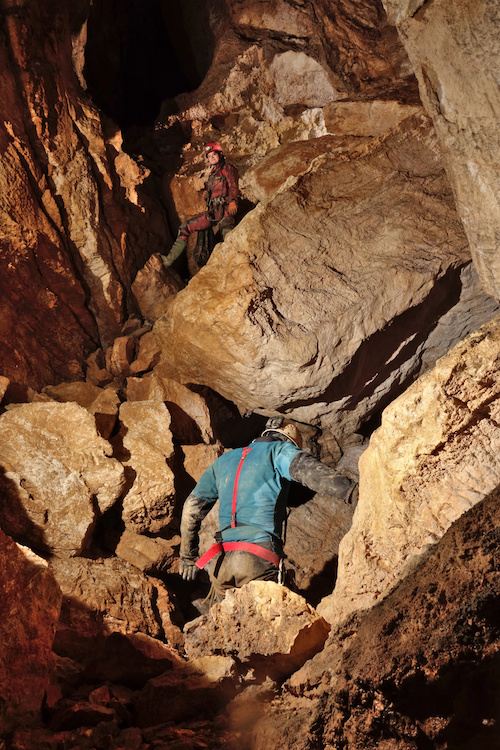
\includegraphics[width=\paperwidth]{backgrounds/RhysTyers-SpiralClimb.jpg}
 					}
	}
\BgThispage
